% LightBanglaHC --- Springer LNCS conference version.
% Converted and compressed from the Elsevier CAS assembly (32 pp.) to the LNCS
% 12-page limit. No new experiments, results, citations, or author facts were
% introduced during the conversion. Evidence markers are retained deliberately
% and must not be removed by cosmetic editing.
\documentclass[runningheads]{llncs}

\usepackage[T1]{fontenc}
\usepackage{newtxtext}
\usepackage[varvw]{newtxmath}
\usepackage{graphicx}
\usepackage{amsmath}
\usepackage{booktabs}
\usepackage{array}
\usepackage{tabularx}
\usepackage{url}
\urlstyle{sf}

\newcolumntype{P}[1]{>{\raggedright\arraybackslash}p{#1}}
\newcommand{\needexp}{\textbf{[REQUIRES NEW EXPERIMENT]}}
\newcommand{\verifyauthor}{\textbf{[AUTHOR TO VERIFY]}}
\newcommand{\notestablished}{\textbf{[NOT ESTABLISHED BY AVAILABLE EVIDENCE]}}

\begin{document}

\title{LightBanglaHC: Evaluation Validity, Inference\\Reconstruction, and Accounting Boundaries in\\Harmful-Content Classification}

% \titlerunning{Evaluation Validity and Accounting Boundaries}

% AUTHOR BLOCK --- INTENTIONALLY UNFILLED.
% The source package supplied no verified authorship, and author facts must not
% be inferred from chats, filenames, or code commits. Replace the fields below
% with verified names, affiliations, and ORCIDs before submission.
\author{\verifyauthor{} Author Name\inst{1}\orcidID{0000-0000-0000-0000}}
% \authorrunning{\verifyauthor{} Author et al.}
\institute{\verifyauthor{} Institution, City, Country\\
\email{corresponding.author@institution.example}}

\maketitle


\begin{abstract}
Evaluating the efficiency of a harmful content classifier requires separating a small prediction component from the complete pipeline that produces its inputs. We study this separation through a retrospective audit of LightBanglaHC, a recorded implementation from the HerWILL AI for Digital Safety Datathon 2026. The recorded run uses 47,817 labeled training examples, 11,955 unlabeled test rows, and three classes defined by the implementation. Its 254,983 concatenated TF-IDF features feed four classical classifier families and two alternative linear stackers. A PyTorch linear head records the highest pooled out-of-fold macro-F1, 0.5295, compared with 0.5246 for logistic regression. This gap is descriptive and does not show superior performance. Globally fitted transformations and class weights, nonnested meta validation, and checkpoint and candidate selection all connect fitting to the reported scores. A dependency analysis of the source code shows why excluding each row from its own base fit does not isolate the full stacking procedure. The reported 39 parameters also describe only one head. The test procedure averages five heads, or 195 parameters, and the five logistic regression fits on the same path imply 3,824,760 coefficients and intercepts. We label each claim by its evidence type and specify a corrected protocol for evaluation and resource measurement. Overall, the study provides an inspectable case study of alignment among inference, evaluation, and accounting, rather than introducing a new classification algorithm or demonstrating a deployment advantage.

% Resource-conscious evaluation of harmful-content classifiers must distinguish a
% small classifier component from the complete predictor: the efficiency of a
% sparse system cannot be established by counting a combination head while
% excluding the fitted representations and estimators that produce its inputs. We
% examine this alignment problem through a retrospective case study of
% LightBanglaHC, a recorded implementation associated with the HerWILL AI for
% Digital Safety Datathon 2026, whose notebook records 47,817 training examples,
% 11,955 test rows, three implementation-defined classes, and 254,983 concatenated
% TF--IDF features feeding four classical classifier families and two alternative
% linear stackers. A PyTorch linear head attains the highest selected pooled
% out-of-fold macro-F1, 0.5295, against 0.5246 for logistic regression, but the
% difference is descriptive rather than independently validated: globally fitted
% transformations and class weights, nonnested meta-validation, and checkpoint and
% candidate selection connect fitting to the reported outcomes, and a source-level
% dependency analysis explains why row-wise out-of-fold exclusion does not isolate
% the complete stacking procedure. Parameter accounting establishes 39 scalars in
% one head and 195 across the five heads averaged at test time, while the five
% logistic-regression fits on the same path imply 3,824,760 coefficients and
% intercepts. Separating source observations, recorded outputs, arithmetic
% reconstructions, unverified external scores, and prospective experiments, we
% specify a corrected evaluation and measurement protocol. The contribution is an
% inspectable case study of inference, evaluation, and accounting alignment, not a
% new algorithm or a demonstrated deployment advantage.

\keywords{Harmful-content classification \and Evaluation validity \and Stacked
generalization \and Accounting boundaries \and Reproducibility.}
\end{abstract}



\section{Introduction}
\label{sec:introduction}

Harmful content classification is usually judged by a single performance number. That number only makes sense once we know the full procedure that produced it. Labels in this task encode interpretive decisions about which expressions count as harmful, so both the metric and the system behind it need careful description. This matters most for systems built under tight resources, where a reported model size may cover only one part of a larger prediction pipeline. In sparse and ensemble classifiers, a final prediction can depend on learned representations, several base estimators, calibration steps, and a second-stage prediction head. Claims about accuracy and efficiency are meaningful only when the evaluated object and the reported quantity are stated explicitly.

We describe this separation with three related objects. The \emph{inference object} is the full computation that turns raw text into a prediction. The \emph{evaluation object} is the training, validation, and selection procedure that produces the predictions behind a reported metric. The \emph{accounting object} is the defined set of artifacts and computations included in a resource or model size statement. These objects need not coincide. Reporting the parameter count of a small neural head does not describe the inference system if that head runs on a large fitted representation and several upstream estimators. This gap matters for resource-conscious machine learning, where cost and efficiency should be reported together with predictive performance~\cite{schwartz2020greenai}.

The distinction is especially important for stacked models. Stacking feeds the predictions of base learners into a second-level learner~\cite{wolpert1992stacked}. Out-of-fold (OOF) predictions are often used to avoid direct contamination between training and validation. However, excluding rows one at a time does not guarantee that the whole stacking pipeline is isolated. A meta training feature can carry labels from a partition that the same base models later treat as meta validation. Globally fitted transformations and repeated model selection can also create dependencies that fold assignment does not reveal. These concerns follow established work on model selection bias and overfitting~\cite{varma2006bias,cawley2010overfitting} and more recent work on leakage in machine learning evaluation~\cite{kapoor2023leakage}. An evaluation should therefore be judged by the dependency structure of the full procedure, not only by checking that each validation row was excluded from the model that predicted it.

We study these questions through a retrospective audit of LightBanglaHC, a recorded implementation from the 2026 HerWILL AI for Digital Safety Datathon. The analysis uses one supplied notebook run, its source code, and its stored aggregate outputs. The raw CSV files, row level predictions, and fitted model artifacts are not available. We therefore do not rerun training and do not verify the recorded outputs against the original data. The analysis focuses on what the available artifacts establish and on explicit reconstructions built from them. Bangla aware preprocessing is not treated as evidence of a Bangla only corpus or of language specific performance. The class names assigned in code are not treated as a substitute for an annotation manual.

Within these limits, the paper reconstructs the executed inference pipeline and identifies the components its predictions depend on. It then analyses the dependency structure of the selected OOF evaluation and explains why row level exclusion alone does not isolate the full stacking procedure. It examines the boundary behind the reported parameter count and separates the final prediction head from the upstream state required at inference. It closes with a prospective protocol for more rigorous evaluation and resource measurement. The study does not claim algorithmic priority, superiority of transformer models, or validated deployment efficiency.

Each claim carries an evidence type: S (source observation), R (recorded output, which verifies what the artifact records but not its authenticity against raw data), A (arithmetic reconstruction), X (external unverified quantity), or P (prospective proposal). Missing empirical evidence is marked \textbf{[REQUIRES NEW EXPERIMENT]}. Missing source, governance, or author information is marked \textbf{[AUTHOR TO VERIFY]}. Unsupported conclusions are marked \textbf{[NOT ESTABLISHED BY AVAILABLE EVIDENCE]}. These markers are retained deliberately and must not be removed by cosmetic editing.

Section~\ref{sec:related} reviews related work. Section~\ref{sec:design} describes the study design and evidence base. Sections~\ref{sec:pipeline} and~\ref{sec:record} reconstruct the pipeline and its experimental record. Section~\ref{sec:validity} analyses evaluation validity, and Section~\ref{sec:accounting} analyses parameter and resource accounting. Section~\ref{sec:discussion} discusses limitations and the corrected protocol, and Section~\ref{sec:conclusion} concludes.
















% To maintain a clear separation between evidence and inference, claims throughout the paper are explicitly labeled as \textbf{S} (source observation), \textbf{R} (recorded output, describing what the artifact records rather than independently authenticating it), \textbf{A} (arithmetic reconstruction), \textbf{X} (an external quantity that could not be independently verified), or \textbf{P} (prospective proposal). Missing empirical evidence is marked \needexp; missing source, governance, or author information is marked \verifyauthor; and conclusions that are not supported by the available evidence are marked \notestablished. These labels are preserved to make the audit’s evidentiary boundaries explicit, rather than to suggest validation that was not carried out.

% Harmful-content classification joins a predictive problem to a problem of
% interpretation: labels encode decisions about which expressions count as harmful
% and when. Offensive vocabulary, hostility toward an individual, and attacks on a
% social group are not interchangeable constructs, as the distinction between hate
% speech and offensive language~\cite{davidson2017automated} and the separate
% dimensions of directness, hostility type, and
% target~\cite{ousidhoum2019multilingual} show. Because Bangla text classification already
% spans sparse models, ensembles, pretraining, and code-mixed
% representations~\cite{romim2022bdshs,tripty2025cuet,bhattacharjee2022banglabert,raihan2024mixeddistilbert},
% a sparse system cannot be motivated by an absence of alternatives; what is needed
% is precision about the representation, prediction path, and resource boundary
% under comparison.

% We frame this as alignment among three objects: the \emph{inference object}, the
% complete computation turning raw text into the reported prediction; the
% \emph{evaluation object}, the training-and-selection procedure whose predictions
% the reported metric evaluates; and the \emph{accounting object}, the delimited
% set of artifacts included in a cost statement. Counting a neural head omits the
% vocabulary, IDF weights, calibrated base estimators, and additional heads its
% predictions depend on, even though Green AI motivates reporting expenditure
% alongside accuracy~\cite{schwartz2020greenai}. This matters most in stacking: held-out base predictions are useful training inputs for a
% second-level learner~\cite{wolpert1992stacked}, but their out-of-fold (OOF)
% status does not make every subsequent use an independent evaluation, because a
% meta-training feature can depend on labels from a partition later treated as
% meta-validation. Global fitting and repeated selection create further paths that
% a fold label does not reveal, which is why work on model-selection
% bias~\cite{varma2006bias,cawley2010overfitting} and
% leakage~\cite{kapoor2023leakage} motivates inspecting the complete procedure.

% The case is LightBanglaHC, developed for the 2026 HerWILL AI for Digital
% Safety Datathon. We analyse one supplied notebook execution, its source, and
% preserved aggregate outputs; training is not rerun and the outputs are not
% authenticated against original rows, since the raw CSVs, row-level predictions,
% and fitted artifacts are unavailable. Bangla-aware preprocessing establishes
% neither a Bangla-only corpus nor any language-specific performance, and the class
% names are code-assigned descriptors, not an annotation manual. The paper
% contributes an evidence-aware reconstruction of the
% executed pipeline, a dependency analysis of the selected OOF result, a scoped
% accounting analysis separating one head from the retained ensemble and upstream
% state, and a prospective protocol, while claiming neither algorithmic priority,
% transformer superiority, nor validated resource savings. Claims are tagged
% \textbf{S} (source observation), \textbf{R} (recorded output, verifying what the
% artifact records rather than its authenticity against raw data), \textbf{A}
% (arithmetic reconstruction), \textbf{X} (external unverified quantity), or
% \textbf{P} (prospective proposal); missing empirical evidence is marked
% \needexp, missing source, governance, or author information \verifyauthor, and
% unsupported conclusions \notestablished. These markers are retained deliberately
% and must not be removed by cosmetic editing.











% \section{Related Work and the Scoped Research Gap}
% \label{sec:related}

% Taxonomy determines what a classification error means, and neither the three-way
% English scheme of~\cite{davidson2017automated} nor the multi-aspect scheme
% of~\cite{ousidhoum2019multilingual} maps onto LightBanglaHC's explicit, subtle,
% and neutral classes: ``subtle'' is not evidence of a validated sarcasm category.
% BD-SHS is the closest linguistic context, pairing Bangla hate-speech
% identification with target and type annotations and evaluating linear SVMs over
% word and character TF--IDF features~\cite{romim2022bdshs}, but no verified
% provenance connects it to the HerWILL data, so collection context remains an
% evidence requirement, not an inherited fact~\cite{bender2018datastatements}.
% Sparse classifiers are meaningful controls when their features and estimator
% variants are specified, since Complement Naive Bayes derives from a distinct
% complement-class estimation~\cite{rennie2003tackling} and voting designs use
% comparable representations for Bengali hate speech~\cite{tripty2025cuet}; yet
% sparsity guarantees neither accuracy nor low deployment cost, because sparse
% inputs coexist with large coefficient arrays and many retained estimators. Stacked generalization learns a fitted
% second-level predictor from base-model outputs~\cite{wolpert1992stacked}, and
% one precedent pairs classical first-level learners with a neural second-level
% classifier for Bangla religious-hate comments~\cite{hasan2024religioushate},
% establishing lineage rather than equivalence.

% Evaluation must also include adaptive choices, since cross-validation used both
% to choose settings and to estimate their error is
% biased~\cite{varma2006bias,cawley2010overfitting}; probability quality is a
% separate requirement~\cite{niculescumizil2005probabilities,vaicenavicius2019calibration};
% uncertainty cannot be recovered by treating folds as independent
% replications~\cite{bengio2004variance,dror2018significance}; and reproducibility
% requires code, reporting, and independent checking
% together~\cite{pineau2021reproducibility}, with model
% cards~\cite{mitchell2019modelcards} recording explicit unknowns, as a recent
% end-user audit of ADMET leaderboard models also
% illustrates~\cite{koleiev2026audit}. The gap addressed here is not universal
% neglect of these topics, but that the interaction among inference scope,
% evaluation ancestry, and accounting boundaries has not been made inspectable
% within one recorded harmful-content artifact.


\section{Related Work}
\label{sec:related}

Automated harmful content classification is a broad area. It encompasses how harm is defined, how labeled resources are built, how models are designed, and how those models are evaluated. This review narrows the scope to sparse, stacked classifiers for Bangla and to the methods used to describe and assess them. The topic is important because such systems are frequently adopted in low-resource settings based on claims of accuracy and efficiency. If those claims refer to a different computation than the one underlying the predictions, then both the scientific conclusions and any subsequent deployment choices are grounded in the wrong object. The review is organized around three questions: Which computation does a reported prediction actually depend on? Does out-of-fold stacking fully separate the training and selection process from its evaluation labels? And does a reported parameter count correspond to the computation whose predictions were scored? Rather than being systematic, the review is selective. We include work that defines the harmful content constructs against which our class names must be compared, work that builds Bangla harmful content resources or models, methodological studies on selection bias, leakage, calibration, and uncertainty, and work on reporting and resource accounting. We exclude English-only architecture papers except as contrast, and we exclude moderation policy and legal literature because this audit makes no deployment claim. Section~\ref{sec:rw-constructs} addresses constructs and taxonomies. Section~\ref{sec:rw-bangla} covers Bangla resources and models. Section~\ref{sec:rw-stacking} discusses sparse classifiers and stacking. Section~\ref{sec:rw-eval} considers evaluation validity. Section~\ref{sec:rw-accounting} covers resource accounting and reporting.

\subsection{Constructs and Taxonomies of Harmful Content}
\label{sec:rw-constructs}
"Harmful content" is an umbrella term, and the constructs beneath it are not interchangeable. Offensive vocabulary, hostility aimed at an individual, and attacks on a social group are distinct phenomena, and a scheme that separates them allows an error to be interpretable \citationneeded{hate speech vs offensive language taxonomy}. Schemes that annotate multiple dimensions simultaneously—such as directness, hostility type, and target—make this separation even more granular \citationneeded{multi-aspect hate speech annotation}. Under such schemes, an error has a specific meaning. Mistaking offensive text for hateful text represents a different kind of failure than failing to identify a target group.

LightBanglaHC’s explicit, subtle, and neutral classes do not correspond to either of these scheme types. Without an annotation manual, the label "subtle" cannot be interpreted as a validated category of sarcasm or implicitness, and confusion between explicit and subtle therefore cannot be understood as a construct error. Functional testing sharpens this concern: detection models fail on counter speech, negation, and reclaimed slurs, which are precisely the cases where lexical cue matching is least reliable \citationneeded{functional testing for hate speech models}. Research on how bias is framed in natural language processing makes the same point from a different angle, by asking which harms a system addresses and for whom \citationneeded{critical survey of bias in NLP}. Accordingly, the meaning of a harmful content metric depends on a documented construct, and competition releases often do not provide one.

\subsection{Bangla Harmful Content Resources and Models}
\label{sec:rw-bangla}

Bangla harmful content detection already has benchmark resources that map hate-speech labels to target and type annotations, and that assess linear classifiers using word and character TF-IDF features \citationneeded{Bangla hate speech benchmark dataset}. As a result, sparse models are treated as a well-established reference point in this line of work rather than as an untested default. Pretrained models provide strong alternatives, including monolingual Bangla pretraining \citationneeded{Bangla pretrained language model} and code-mixed modelling for text that combines Bangla with English \citationneeded{code-mixed Bangla modelling}. Ensemble and hierarchical approaches have also been used for Bengali hate speech in shared tasks \citationneeded{Bengali hate speech shared task ensemble}.

A sparse system, then, cannot be justified solely by the lack of alternatives. Its rationale must rest on a specific account of the representation, the prediction pathway, and the cost bound being compared. Provenance is a separate issue. No verified link connects any public Bangla resource to the HerWILL data. Documentation practices that record curation rationale, language variety, and annotator background exist precisely for this purpose \citationneeded{dataset documentation practice}. Without such documentation, a result remains dependent on the access context instead of being attributable to a known population.

\subsection{Sparse Classifiers, Ensembles, and Stacking}
\label{sec:rw-stacking}

Sparse linear models continue to be valuable controls when their features and estimator variants are explicitly specified. Complement Naive Bayes estimates parameters from the complement of each class, making it a distinct estimator rather than a minor variation of the multinomial formulation \citationneeded{Complement Naive Bayes}. The behaviour of these estimators also depends on library defaults \citationneeded{scikit-learn}, which is why version information is important for any attempt at reconstruction. Sparsity alone does not guarantee low deployment cost. Sparse inputs can coexist with large dense coefficient arrays and many retained estimators.

Stacked generalization trains a second-level learner on held-out predictions produced by base learners, enabling the combiner to learn how those learners make errors on unseen data~\cite{wolpert1992stacked}. Combining conventional first-level learners with a neural second-level classifier is a known pattern in Bangla harmful content \citationneeded{stacked ensemble for Bangla hate comments}, which gives LightBanglaHC’s design a lineage but not an equivalence. Calibration introduces an additional fitted layer. Different learners systematically distort probabilities in characteristic ways, and isotonic or sigmoid calibration compensates for that distortion \citationneeded{calibration of classifier probabilities}. When calibrated probabilities are supplied to a meta learner, the calibrators become part of the inference object. Coverage in this area typically reports the accuracy of the meta learner. It seldom describes the fitted state of every base model or the complete lineage of the features used for meta training.

\subsection{Evaluation Validity: Selection, Leakage, and Uncertainty}
\label{sec:rw-eval}

A substantial body of research indicates that the process used to produce an estimate can systematically bias it. Using cross validation both to select a model and to estimate its error yields overly optimistic estimates, whereas nested cross validation produces estimates that are nearly unbiased~\cite{varma2006bias}. Bias can also arise when the model-selection criterion is overfit, potentially reaching magnitudes as large as the differences between the algorithms being compared~\cite{cawley2010overfitting}. Leakage has been documented across many scientific domains, including situations in which preprocessing is fit on data later used for evaluation~\cite{kapoor2023leakage}. Retrospective reviews of leaderboard entries show that a reported artifact can be examined after the fact to assess reproducibility, leakage, and overfitting \citationneeded{end-user audit of leaderboard models}, which is the closest methodological counterpart to the present study.

Uncertainty and probability quality are distinct requirements. Fold scores should not be treated as independent replications, because there is no unbiased estimator for the variance of K fold cross validation \citationneeded{variance of K-fold cross-validation}. Significance testing in natural language processing requires paired predictions, which many report-aggregation procedures often fail to preserve \citationneeded{significance testing in NLP}. Calibration calls for its own dedicated evaluation, since accuracy-based metrics do not capture it \citationneeded{evaluating model calibration}. Much of this literature focuses on single models or on global preprocessing. In the harmful content literature, the specific route by which meta validation labels pass into meta training features through base fits is seldom made explicit.

\subsection{Resource Accounting and Reporting}
\label{sec:rw-accounting}

Efficiency should be reported together with accuracy, including parameter counts and operation counts among the candidate measures~\cite{schwartz2020greenai}. Reporting frameworks for energy and carbon costs further show that parameters, runtime, and energy are separate quantities that cannot substitute for one another \citationneeded{energy and carbon reporting framework}. On the reproducibility front, code submission, reporting checklists, and independent review operate jointly rather than in isolation \citationneeded{reproducibility program report}, and structured model documentation provides a venue for recording intended use, evaluation conditions, and known unknowns \citationneeded{model cards}. This guidance specifies what information to report. It says less about how to draw the boundary when the portion being counted is a small head that runs on a large fitted state.

\subsection{Summary and Research Gap}
\label{sec:rw-summary}

The literature supports several conclusions. Constructions in harmful content must be documented before errors can be properly interpreted. Bangla offers both sparse and pretrained options, so choosing sparse features requires an explicit justification. Stacking depends on held-out predictions~\cite{wolpert1992stacked}. Evaluating adaptive selection and leakage bias~\cite{varma2006bias,cawley2010overfitting,kapoor2023leakage}. Efficiency claims require a clearly defined boundary~\cite{schwartz2020greenai}.

Three gaps remain particularly relevant here. Competition datasets often omit construct and provenance documentation, meaning that label semantics cannot be recovered from class names. In harmful content work, the evaluation lineage of stacked meta features is rarely traced, so an out-of-fold label is treated as sufficient evidence of proper isolation. Guidance on accounting does not resolve the mismatch between a counted head and the full predictor. The gap addressed by this paper is not simply that these topics are handled separately. Rather, it is that their interaction has not been made inspectable within a single recorded harmful content artifact. Section~\ref{sec:discussion} lays out a protocol that addresses these gaps prospectively.

















% \section{Study Design, Evidence, and Dataset Scope}
% \label{sec:evidence}

% This is a retrospective, single-artifact audit whose unit of analysis is the
% relationship between an implementation, its recorded outputs, and the claims
% those materials support. The supplied notebook contains one code cell, 1,248
% source lines, an execution count of one, two saved standard-output streams, and
% an embedded figure, with metadata dating the run to 18 April 2026. We identify invoked fitting, prediction, selection, and saving operations by
% following their inputs rather than descriptive comments, check saved outputs
% against identities such as class-support totals and confusion-matrix margins,
% and assign each claim an evidence type. Findings are restricted to the inspected
% artifact, whose SHA-256 digests are \texttt{5a7ea479\ldots38aeedc0} and
% \texttt{675e2638\ldots6acf1a8287}; its raw CSVs, row-level predictions, and
% fitted artifacts are absent, so corpus statistics, vocabularies, individual
% predictions, and reload equivalence cannot be checked.

% The task assigns one of three labels to an input text, the saved shapes being
% $(47{,}817,3)$ and $(11{,}955,2)$ before the processed-text column is added. The
% recorded supports (R) are 23,756 Explicit Toxic, 18,163 Subtly Toxic, and 5,898
% Neutral, or 49.681\%, 37.984\%, and 12.335\% (A), giving balanced weights
% 0.670946, 0.877553, and 2.702442 (A) under $w_c=n/(3n_c)$, computed once from all
% training labels before cross-validation; the 11,955 unlabeled test rows are not
% an evaluated sample. The competition-named input path identifies an access
% context, not a population: collection dates, annotation instructions, annotator
% agreement, duplicate structure, language composition, and licensing and consent
% records are unavailable, so recovering them is prospective (P) and their absence
% is an evidence gap rather than a negative finding. The reported metric is the
% unweighted mean of the three classwise F1 values, pooled after assembling one
% prediction per training row; because F1 is nonlinear in confusion counts, that
% value need not equal the mean of fold values.


\section{Study Design, Evidence, and Dataset Scope}
\label{sec:design}

\subsection{Design and Questions}

This retrospective audit focuses on a single artifact. Rather than analyzing a model, it treats a relationship as the unit of analysis: the connection among an implementation, the outputs it produced, and the claims that those materials support. The audit poses three questions about the recorded run. On which computation do the reported predictions rely? Does the selected out-of-fold procedure disentangle fitting and selection from the labels used to evaluate them? Does the reported parameter count correspond to the computation whose predictions were scored?

Each question targets a different object. The first addresses the inference object, the second the evaluation object, and the third the accounting object. The audit does not ask whether the system performs well. Because this cannot be determined from the available materials, treating it as answerable is the mistake the paper investigates.

\subsection{Audit Method}

We examine the source to determine what was actually invoked, not what the authors intended. Fitting, prediction, selection, and saving operations are identified by tracing their inputs. Descriptive comments are not treated as evidence of behavior, since a comment may describe a design that the code does not implement.

Next, we verify the saved outputs for internal consistency. Class support totals and confusion matrix margins must match one another and the size of the recorded corpus. Consistency of this kind substantiates what the artifact records. It does not establish that the record matches the original data, and we keep these two assertions distinct throughout.

Every claim is assigned an evidence type. S denotes a source observation. R denotes a recorded output. A denotes an arithmetic reconstruction. X denotes an external quantity that we cannot verify. P denotes a prospective proposal. Claims for which the required evidence is missing are marked with \needexp{}, \verifyauthor{}, or \notestablished{} as appropriate.

\subsection{Available and Missing Artifacts}

The provided notebook contains one code cell and 1,248 source lines. Its execution count is one. It retains two standard output streams and one embedded figure. The metadata dates the run to 18 April 2026. The SHA-256 digests of the inspected files are \texttt{5a7ea479...38aeedc0} and \texttt{675e2638...6acf1a8287}.

Three categories of material are absent: the raw CSV files, the row-level predictions, and the fitted model artifacts. This absence imposes strict constraints on the audit. Corpus statistics cannot be recomputed. Fitted vocabularies cannot be inspected. Individual predictions cannot be reviewed, so no paired comparison between candidates can be performed. Because reload equivalence cannot be evaluated, we cannot confirm that the recorded pipeline would reproduce its own outputs in a fresh process. As a result, the findings are limited to the inspected artifact.

\subsection{Task and Recorded Corpus}

The task assigns one of three labels to an input text. The saved array shapes are (47,817, 3) for the training data and (11,955, 2) for the test data, recorded before the processed text column is added. Table~\ref{tab:supports} gives the recorded class supports with the proportions and class weights derived from them.

\begin{table}[t]
\centering
\caption{Recorded training class supports (R) with proportions and balanced class weights reconstructed from those counts (A). Weights follow $w_c = n/(3n_c)$ and were computed once from all training labels before any fold was constructed.}
\label{tab:supports}
\begin{tabular}{lrrr}
\toprule
Class & Support & Proportion (\%) & Weight \\
\midrule
Explicit Toxic & 23,756 & 49.681 & 0.670946 \\
Subtly Toxic & 18,163 & 37.984 & 0.877553 \\
Neutral & 5,898 & 12.335 & 2.702442 \\
\midrule
Total & 47,817 & 100.000 & \\
\bottomrule
\end{tabular}
\end{table}

The timing of the weight computation matters for what follows. The weights were derived from every training label before cross-validation began, so each fold was fitted under weights that depend on the class counts of the fold used to score it. Section~\ref{sec:validity} traces the consequence. The 11,955 test rows carry no labels. They are not an evaluated sample, and predictions on them support no accuracy claim.

\subsection{Dataset Scope}

The input path names a competition, which specifies an access context rather than a population. Collection dates, annotation instructions, annotator agreement, duplicate structure, language composition, and licensing and consent records are all unavailable. Recovering them is prospective (P). Their absence is an evidence gap, not a negative finding, and we do not treat it as criticism of the original release.

Therefore, two inferences cannot be drawn. Bangla-aware preprocessing does not yield a Bangla-only corpus, and the three class names used in the code cannot replace an annotation manual.



\subsection{Reported Metric}

The reported metric is the unweighted mean of the three classwise F1 values. It is obtained through pooling: for each training row, a single prediction is generated, and the metric is computed once on the resulting pooled set. Pooling is not averaging. Because F1 is nonlinear with respect to the confusion counts, the pooled value is not required to match the mean of the five-fold values, and the two quantities should not be treated as if they captured the same measurement.









% \section{Recorded LightBanglaHC Pipeline}
% \label{sec:pipeline}

% Let $x$ be the original string after missing-value handling. The processed string
% is $s(x)=C(x)\mathbin{\Vert}\texttt{ FEATSEP }\mathbin{\Vert}H(x)$, where $C$
% cleans and $H$ emits synthetic tokens. Crucially $H$ receives $x$, not $C(x)$, so
% the cleaner's normalization, lowercasing, and token replacements neither erase
% the original capitalization and punctuation before feature extraction nor
% normalize the input used by the lexical rules. The injector holds 42 explicit
% lexical entries, 14 subtle-pattern expressions, and nine sarcasm-pattern
% expressions (S), each counted once per matching entry, and emits capped markers
% for lexical hits, script mixture, capitalization, length, punctuation, emoji, and
% whole-word religious, gender, or threat cues, with no context or intent
% validated. Those names are code identifiers, not measured constructs: ``this is
% a salad'' triggers the entry \texttt{sala}.

% For branch $r$, with $t_{ij}^{(r)}$ the count of retained feature $j$ in
% processed document $i$, $\mathrm{df}_j^{(r)}$ its document frequency, and $N$ the
% number of fitting documents, the documented-default interpretation of the omitted
% normalization and IDF options gives
% \begin{equation}
% u_{ij}^{(r)}=
% \bigl(1+\ln t_{ij}^{(r)}\bigr)
% \Bigl[1+\ln\tfrac{N+1}{\mathrm{df}_j^{(r)}+1}\Bigr]
% \ \text{ for } t_{ij}^{(r)}>0,
% \qquad
% \phi_r(x_i)=u_i^{(r)}/\lVert u_i^{(r)}\rVert_2 ,
% \label{eq:tfidf}
% \end{equation}
% and $u_{ij}^{(r)}=0$ otherwise. The source sets sublinear TF for all branches and
% smoothed IDF for the word branch but leaves normalization and the
% character-branch DF and IDF options unset, so historical behaviour and the fitted
% arrays remain \verifyauthor.\footnote{Consulted API: \url{https://scikit-learn.org/1.5/modules/generated/sklearn.feature_extraction.text.TfidfVectorizer.html};
% this documentation version is not evidence of the historical runtime version.}
% The branches are configured (S) as a word analyzer over non-whitespace tokens
% with 1--4-grams, a 150,000-feature cap and document frequency in $[1,0.98]$; a
% \texttt{char\_wb} analyzer with 2--6-grams and a 100,000-feature cap; and a
% \texttt{char} analyzer with 1--2-grams and a 50,000-feature cap, both requiring
% two documents. Their sparse concatenation has the only recorded width
% $D=254{,}983$ (R); the caps sum to 300,000, but individual fitted widths are
% unlogged, so assigning widths 150,000, 100,000, and 4,983 would be unsupported.
% All three vectorizers are fitted to the entire training corpus before folds are
% constructed, so $\phi$ is a global map and later label exclusion is not
% representation isolation.

% Table~\ref{tab:models} lists the invoked configurations. Complement Naive Bayes
% (CNB) uses only \texttt{char\_wb} features~\cite{rennie2003tackling}; a source
% comment ties that restriction to nonnegativity, but all three branches are
% nonnegative, so the choice is an implementation fact rather than an ablated
% design. Isotonic calibration of CNB, LinearSVC (SVC), and SGDClassifier (SGD)
% changes the probability-generating procedure supplied to the
% meta-model~\cite{niculescumizil2005probabilities} and inherits globally fitted
% features and class weights, and no diagnostic is
% recorded~\cite{vaicenavicius2019calibration}.

% \begin{table}[tb]
% \centering\footnotesize
% \caption{Verified invoked configurations (S). Unspecified arguments retain library defaults; installed library versions and fitted calibrator internals are unavailable.}
% \label{tab:models}
% \begin{tabularx}{\textwidth}{@{}P{0.115\textwidth}P{0.125\textwidth}>{\raggedright\arraybackslash}X@{}}
% \toprule
% Candidate & Inputs & Explicit settings and training controls \\
% \midrule
% LR & Full TF--IDF & $C=8$; \texttt{saga}; multinomial; max.\ 2,000 iterations;
% tolerance $10^{-4}$; global balanced weights; seed 42. \\
% CNB & \texttt{char\_wb} & $\alpha=0.05$; \texttt{norm=True}; isotonic
% calibration, CV${}={}$3; no explicit class-weight argument. \\
% SVC & Full TF--IDF & $C=0.3$; max.\ 5,000 iterations; \texttt{dual=True}; global
% balanced weights; seed 42; isotonic calibration, CV${}={}$3. \\
% SGD & Full TF--IDF & Modified-Huber loss; $\alpha=10^{-4}$; max.\ 200 iterations; tolerance $10^{-4}$; global balanced weights; seed 42; isotonic calibration, CV${}={}$3. \\
% Meta-LR & 12 probabilities & $C=10$; max.\ 500 iterations; multinomial; global
% balanced weights; seed 42; solver not explicitly overridden. \\
% TinyLinear & 12 probabilities & Linear(12,3); Xavier-uniform weights; weighted cross-entropy; AdamW rate 0.005, decay $10^{-4}$; cosine scheduler $T_{\max}=30$; max.\ 30 epochs; patience 8; batches 512/1,024; seeds 42--46. \\
% \bottomrule
% \end{tabularx}
% \end{table}

% Let $V_1,\dots,V_5$ be disjoint validation sets partitioning $I=\{1,\dots,n\}$
% from shuffled stratified five-fold splitting with seed 42, and let $f(i)$ be the
% fold containing $i$. For family $b$, $h_b^{(-f)}$ is its probability-producing
% fit on $I\setminus V_f$, including calibration where applicable, with the global
% $\phi$ as input; the superscript excludes $V_f$ from estimator fitting, not from
% vocabulary estimation or weight computation. The meta-training row and the
% test-time feature vector are
% \begin{equation}
% z_i=\bigl[h_b^{(-f(i))}(\phi(x_i))\bigr]_{b=1}^{4}\in\mathbb{R}^{12},
% \qquad
% \bar z(x)=\Bigl[\tfrac{1}{5}\textstyle\sum_{f=1}^{5}h_b^{(-f)}(\phi(x))\Bigr]_{b=1}^{4},
% \label{eq:oof}
% \end{equation}
% so training rows receive one fold-specific base prediction per family while test
% rows receive within-family averages. TinyLinear computes logits $\ell_i=Wz_i+b$
% with $W\in\mathbb{R}^{3\times12}$ and no hidden layer, trained with weighted
% cross-entropy; that objective is not macro-F1, which is used instead for
% checkpoint selection, with every epoch assessed on the same fold later included
% in reported validation performance. Final test labels are
% $\widehat y(x)=\arg\max_{c}\frac{1}{5}\sum_{f=1}^{5}q_f(\bar z(x))_c$ over the
% selected heads $q_f$: five softmax outputs averaged, not one head obtained by
% averaging coefficients, implying 39 scalar weights and biases per head and 195
% across five heads (A) before upstream state. Figure~\ref{fig:pipeline} summarises that
% computation, which is not fully nested: when $V_f$ is a meta-validation set, a
% meta-training row in another $V_g$ was represented by a base fit using labels
% from $V_f$.

% \begin{figure}[tb]
% \centering
% 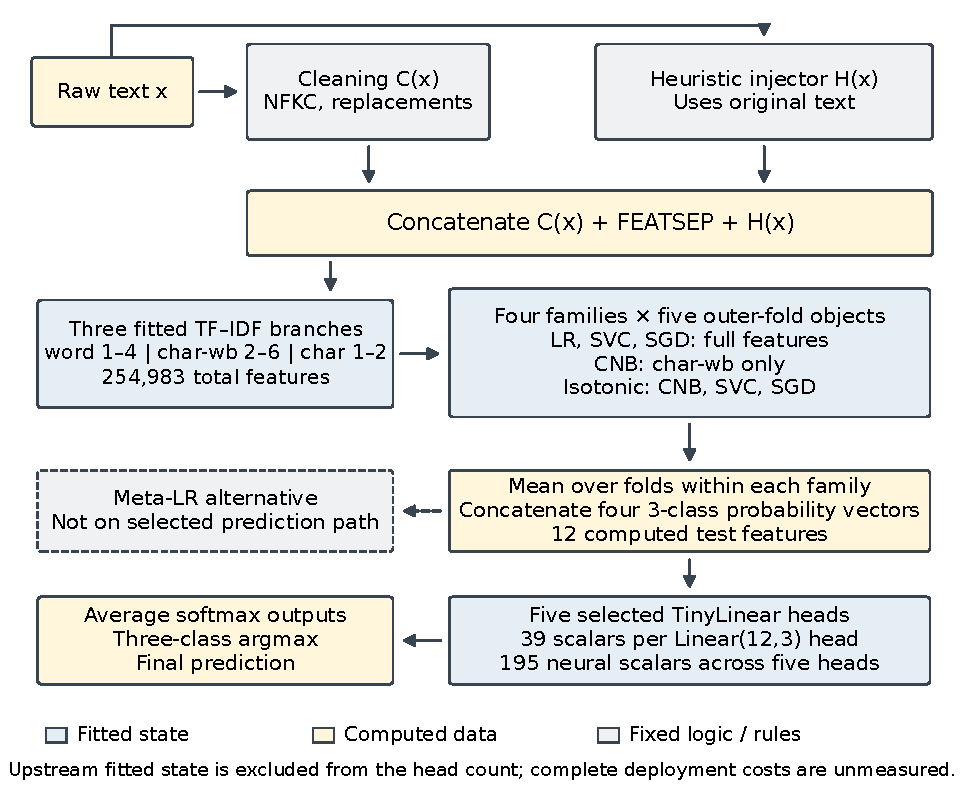
\includegraphics[width=0.68\textwidth]{pipeline.pdf}
% \caption{Source-derived schematic (S), not an experimental plot; the selected path averages five TinyLinear softmax outputs over within-family averages of base-fold predictions.}
% \label{fig:pipeline}
% \end{figure}


\section{Recorded LightBanglaHC Pipeline}
\label{sec:pipeline}

This section reconstructs the computation the notebook executed. The reconstruction follows invoked operations and their inputs. Where a library default governs behaviour that the source leaves unset, we say so and mark the resulting value \verifyauthor{}.

\subsection{Text Processing}

Let $x$ be the original string after missing value handling. The processed string is
\begin{equation}
s(x) = C(x) \,\|\, \texttt{FEATSEP} \,\|\, H(x),
\end{equation}
where $C$ cleans the text and $H$ emits synthetic tokens.

In the definition of $H$, the argument is $x$, not $C(x)$. This distinction holds in both directions. The cleaner’s normalization, lowercasing, and token substitutions do not remove the original capitalization and punctuation prior to feature extraction. Likewise, the lexical rules in $H$ are applied to uncleaned input, so they never observe the normalized form.

The injector contains 42 explicit lexical entries, 14 subtle pattern expressions, and nine sarcasm pattern expressions (S). Each entry is counted once for every match. It outputs capped markers for lexical hits, script mixture, capitalization, length, punctuation, emoji, and full-word cues involving religion, gender, or threats. At no point are any context or intent conditions validated.

The marker names are code identifiers rather than measured constructs. The string ``this is a salad'' activates the entry \texttt{sala}. A marker that is labeled for a threat cue performs a substring match and records nothing beyond that.

\subsection{Sparse Representation}

Three TF-IDF branches are fitted. For branch $r$, let $t^{(r)}_{ij}$ be the count of retained feature $j$ in processed document $i$, let $\mathrm{df}^{(r)}_j$ be its document frequency, and let $N$ be the number of fitting documents. Under the documented default interpretation of the omitted normalization and IDF options,
\begin{equation}
u^{(r)}_{ij} = \left(1 + \ln t^{(r)}_{ij}\right)\left[1 + \ln \frac{N+1}{\mathrm{df}^{(r)}_j + 1}\right] \quad \text{for } t^{(r)}_{ij} > 0,
\qquad
\phi_r(x_i) = u^{(r)}_i \big/ \left\|u^{(r)}_i\right\|_2,
\end{equation}
and $u^{(r)}_{ij} = 0$ otherwise.

The source applies sublinear TF across all branches and smoothed IDF for the word branch. It leaves normalization unspecified, and it leaves the character-branch document frequency and IDF options unspecified.\footnote{Consulted API: \url{https://scikit-learn.org/1.5/modules/generated/sklearn.feature_extraction.text.TfidfVectorizer.html}. This documentation version is not evidence of the historical runtime version.} Consequently, historical behavior and the fitted arrays remain \verifyauthor{}.

The branches are configured (S) as follows. The word branch uses an analyzer over non-whitespace tokens with 1 to 4 grams, a 150,000 feature limit, and document frequency in $[1, 0.98]$. The \texttt{charwb} branch uses 2 to 6 grams with a 100,000 feature limit. The \texttt{char} branch uses 1 to 2 grams with a 50,000 feature limit. Both character branches require two documents.

Their sparse concatenation has width $D = 254{,}983$ (R), and this is the only recorded width. The three caps add up to 300,000, but the individual fitted widths are not logged. Therefore, assigning widths of 150,000, 100,000, and 4,983 to the three branches would not be supported.

All three vectorizers are fit on the entire training corpus before any fold is formed. The map $\phi$ is global. As a result, every fold shares a single vocabulary, a single set of document-frequency decisions, and a single set of IDF values, all derived from data that later folds treat as validation. Omitting a row’s label from an estimator does not reverse this, so later label exclusion does not produce representation isolation. Section~\ref{sec:validity} follows what occurs next.

\subsection{Base Families}

Table~\ref{tab:configs} lists the invoked configurations. Complement Naive Bayes (CNB) uses \texttt{char\_wb} features only~\cite{rennie2003tackling}. A source comment attributes this restriction to nonnegativity, but all three branches are nonnegative. The restriction is an implementation fact, not an ablated design choice.


\begin{table}[t]
\centering
\caption{Verified invoked configurations (S). Unspecified arguments retain library defaults. Installed library versions and fitted calibrator internals are unavailable.}
\label{tab:configs}
\begin{tabular}{llP{6.2cm}}
\toprule
Candidate & Inputs & Explicit settings and training controls \\
\midrule
LR & Full TF-IDF & $C = 8$; saga; multinomial; max.\ 2,000 iterations; tolerance $10^{-4}$; global balanced weights; seed 42. \\
CNB & \texttt{char\_wb} & $\alpha = 0.05$; \texttt{norm=True}; isotonic calibration, CV $= 3$; no explicit class weight argument. \\
SVC & Full TF-IDF & $C = 0.3$; max.\ 5,000 iterations; \texttt{dual=True}; global balanced weights; seed 42; isotonic calibration, CV $= 3$. \\
SGD & Full TF-IDF & Modified Huber loss; $\alpha = 10^{-4}$; max.\ 200 iterations; tolerance $10^{-4}$; global balanced weights; seed 42; isotonic calibration, CV $= 3$. \\
Meta-LR & 12 probabilities & $C = 10$; max.\ 500 iterations; multinomial; global balanced weights; seed 42; solver not explicitly overridden. \\
TinyLinear & 12 probabilities & \texttt{Linear(12,3)}; Xavier uniform weights; weighted cross entropy; AdamW rate 0.005, decay $10^{-4}$; cosine scheduler $T_{\max} = 30$; max.\ 30 epochs; patience 8; batches 512/1,024; seeds 42--46. \\
\bottomrule
\end{tabular}
\end{table}


CNB, LinearSVC (SVC), and SGDClassifier (SGD) are isotonically calibrated. Calibration changes the probability generating procedure supplied to the meta model~\cite{niculescu2005predicting}. The calibrators inherit the globally fitted features and the global class weights, and no calibration diagnostic is recorded~\cite{vaicenavicius2019evaluating}.

\subsection{Stacking Construction}

Let $V_1, \dots, V_5$ be disjoint validation sets partitioning $I = \{1, \dots, n\}$, obtained by shuffled stratified five fold splitting with seed 42, and let $f(i)$ be the fold containing $i$. For family $b$, let $h^{(-f)}_b$ be its probability producing fit on $I \setminus V_f$, including calibration where applicable, taking the global $\phi$ as input.

The superscript needs care. It excludes $V_f$ from estimator fitting only. It does not exclude $V_f$ from vocabulary estimation or from the class weight computation, both of which used all training rows.

Training rows and test rows receive their meta features differently:
\begin{equation}
z_i = \left[h^{(-f(i))}_b(\phi(x_i))\right]^4_{b=1} \in \mathbb{R}^{12},
\qquad
\bar{z}(x) = \left[\frac{1}{5}\sum_{f=1}^{5} h^{(-f)}_b(\phi(x))\right]^4_{b=1}.
\end{equation}
A training row receives one fold-specific prediction per family. A test row receives a within-family average over five fits.

TinyLinear computes logits $\ell_i = W z_i + b$ with $W \in \mathbb{R}^{3 \times 12}$ and no hidden layer. It is trained with weighted cross-entropy. That objective is not macro-F1, yet macro-F1 is what selects the checkpoint, and every epoch is assessed on the same fold later included in reported validation performance.

Final test labels are
\begin{equation}
\hat{y}(x) = \arg\max_c \frac{1}{5}\sum_{f=1}^{5} q_f(\bar{z}(x))_c
\end{equation}
over the selected heads $q_f$. Five softmax outputs are averaged. This is not one head obtained by averaging coefficients, and the two are not interchangeable. The construction implies 39 scalar weights and biases per head and 195 across five heads (A), before any upstream state is counted.

Figure~\ref{fig:pipeline} summarises the computation. It is not fully nested. When $V_f$ serves as a meta validation set, a meta training row drawn from another $V_g$ was represented by a base fit that used labels from $V_f$.






\section{Experimental Record}
\label{sec:record}

The record contains six candidate evaluations under one seeded partitioning scheme. This section reports what was recorded and what the recorded values do and do not support.

\subsection{Candidate Comparison}

Table~\ref{tab:results} preserves the pooled and per fold macro-F1 values at their printed precision. TinyLinear is the selected candidate. LR is the strongest base learner.

\begin{table}[t]
\centering
\caption{Recorded pooled out of fold macro-F1 and per fold values (R). All candidates share global feature fitting, and both stackers reuse nonnested out of fold features. Folds are dependent partitions, so no interval is attached.}
\label{tab:results}
\begin{tabular}{llrrrrrr}
\toprule
Candidate & Role & Pooled & Fold 1 & Fold 2 & Fold 3 & Fold 4 & Fold 5 \\
\midrule
LR & Base learner & 0.5246 & 0.5265 & 0.5171 & 0.5259 & 0.5254 & 0.5278 \\
CNB & Base learner & 0.4478 & 0.4501 & 0.4397 & 0.4573 & 0.4468 & 0.4450 \\
SVC & Base learner & 0.5053 & 0.5042 & 0.4950 & 0.5152 & 0.5094 & 0.5027 \\
SGD & Base learner & 0.4977 & 0.4965 & 0.4922 & 0.5049 & 0.5025 & 0.4919 \\
Meta-LR & Alt.\ stacker & 0.5268 & 0.5235 & 0.5183 & 0.5220 & 0.5332 & 0.5369 \\
TinyLinear & Selected stacker & 0.5295 & 0.5264 & 0.5255 & 0.5266 & 0.5338 & 0.5350 \\
\bottomrule
\end{tabular}
\end{table}

The rounded difference between them is 0.0049 macro-F1 (A). Three things limit what that number supports. It is not evidence of stable superiority, since the folds are dependent partitions and no paired predictions were retained. It does not isolate a cause, since TinyLinear and LR differ in probability combination, class weighting, regularization, and stopping rule at once. And it was produced under the shared dependencies described in Section~\ref{sec:pipeline}.

The neural seeds 42 to 46 vary initialization across folds. They are not independent repeated evaluations, and the five resulting scores are not replications of one measurement.

No hyperparameter search is recorded beyond the fixed configurations, the epoch selection, and the six way comparison.

\subsection{Unused Definitions}

Two definitions appear in the source but never execute on the selected path. Neither is an experiment, and neither should be reported as one.

An untrained 12--8--3 MLP is defined. Its parameter count is 131 by arithmetic (A), not the 123 stated in its accompanying comment. A helper carries a learning rate of 0.01. The invoked rate is 0.005, and the helper value must not replace it in any description of the run.

Both cases illustrate the paper's theme at small scale. A recorded number can describe an object the computation never used.

\subsection{Error Structure}

Table~\ref{tab:confusion} reproduces the nine integer annotations of the recorded confusion figure, with classwise metrics reconstructed from those counts. Row sums match all printed supports and total 47,817. The macro-F1 definition yields a pooled value of 0.529547 with accuracy 0.563544 (A).

\begin{table}[t]
\centering
\caption{Selected TinyLinear out of fold confusion matrix (R), with diagonal row percentages and classwise metrics computed from those counts (A). Rows are actual labels and columns predicted labels. Classwise values are rounded from the exact count derived figures.}
\label{tab:confusion}
\begin{tabular}{lrrrrrrr}
\toprule
Actual & Explicit & Subtle & Neutral & Supp. & Prec. & Rec. & F1 \\
\midrule
Explicit & 15,192 (63.95\%) & 6,406 & 2,158 & 23,756 & 0.6790 & 0.6395 & 0.6587 \\
Subtle & 6,217 & 8,509 (46.85\%) & 3,437 & 18,163 & 0.5125 & 0.4685 & 0.4895 \\
Neutral & 964 & 1,688 & 3,246 (55.04\%) & 5,898 & 0.3672 & 0.5504 & 0.4405 \\
\midrule
Predicted (A) & 22,373 & 16,603 & 8,841 & 47,817 & \multicolumn{3}{c}{Macro-F1 0.529547 (A)} \\
\bottomrule
\end{tabular}
\end{table}

Three patterns are visible in the counts. Neutral has the lowest classwise F1, although Subtle has the lower recall. The largest off-diagonal counts are Explicit predicted as Subtle (6,406) and Subtle predicted as Explicit (6,217). Of 8,841 examples predicted Neutral, 5,595 carry a toxic label, while 2,652 actual Neutral examples are assigned one.

These are aggregate counts. They describe where predictions and labels disagree. They establish no cause, and without row level outputs the joint error pattern across candidates cannot be recovered.

An always Explicit predictor would score $\mathrm{MacroF1} = 2n_0 / [3(n + n_0)] = 0.221275$ (A). This is an arithmetic reference point computed from the class supports, not a measured comparison system.

\subsection{Test Predictions and Saved Artifacts}

The test predictions number 5,501 Explicit, 4,139 Subtle, and 2,315 Neutral (R). The test rows carry no labels. These counts are therefore neither an accuracy measurement nor evidence that the class balance of the corpus was recovered.

The source writes a submission with a constant \texttt{parameters} field of 39. It does so without loading the configured sample submission file, so the save message demonstrates neither schema acceptance nor any rank.

Several artifacts needed for replay are missing. The upstream transforms are not serialized. The device string and the Python metadata conflict. Library versions, selected epochs, and fitted state bytes are absent. Section~\ref{sec:accounting} returns to what this means for any resource claim.


% \section{Experimental Record}
% \label{sec:record}

% The record contains six candidate evaluations under one seeded partitioning
% scheme; neural seeds 42--46 vary initialization across folds and are not
% independent repeated evaluations, and Table~\ref{tab:recorded} preserves pooled
% and fold metrics at their printed precision. TinyLinear is the selected candidate
% and LR the strongest base learner, with a rounded difference of 0.0049 macro-F1
% (A) that is not evidence of stable superiority and does not isolate whether it
% arose from probability combination, class weighting, regularization, or stopping.
% No hyperparameter search beyond fixed configurations, epoch selection, and the
% six-way comparison is recorded, and unused definitions are not experiments: the
% untrained 12--8--3 MLP has 131 parameters by arithmetic, not the 123 of its
% comment, and the unused helper rate 0.01 must not replace the invoked 0.005.

% \begin{table}[tb]
% \centering\footnotesize
% \caption{Recorded pooled OOF macro-F1 and per-fold values (R). All candidates share global feature fitting; stackers reuse nonnested OOF features. Folds are dependent partitions, so no interval is attached.}
% \label{tab:recorded}
% \begin{tabular}{@{}llrrrrrr@{}}
% \toprule
% Candidate & Role & Pooled & Fold 1 & Fold 2 & Fold 3 & Fold 4 & Fold 5 \\
% \midrule
% LR & Base learner & 0.5246 & 0.5265 & 0.5171 & 0.5259 & 0.5254 & 0.5278 \\
% CNB & Base learner & 0.4478 & 0.4501 & 0.4397 & 0.4573 & 0.4468 & 0.4450 \\
% SVC & Base learner & 0.5053 & 0.5042 & 0.4950 & 0.5152 & 0.5094 & 0.5027 \\
% SGD & Base learner & 0.4977 & 0.4965 & 0.4922 & 0.5049 & 0.5025 & 0.4919 \\
% Meta-LR & Alt.\ stacker & 0.5268 & 0.5235 & 0.5183 & 0.5220 & 0.5332 & 0.5369 \\
% TinyLinear & Selected stacker & 0.5295 & 0.5264 & 0.5255 & 0.5266 & 0.5338 & 0.5350 \\
% \bottomrule
% \end{tabular}
% \end{table}

% Table~\ref{tab:cm} reproduces the nine integer annotations of the recorded
% confusion figure with classwise metrics reconstructed from them; row sums match
% all printed supports and total 47,817, and the macro-F1 definition yields pooled
% 0.529547 with accuracy 0.563544 (A). Neutral has the lowest classwise F1 although
% Subtle has lower recall, the largest off-diagonal counts are Explicit-to-Subtle
% (6,406) and Subtle-to-Explicit (6,217), and of 8,841 predicted-Neutral examples
% 5,595 carry a toxic label while 2,652 actual-Neutral examples are assigned one;
% these aggregates establish no cause. An always-Explicit predictor would give
% $\operatorname{MacroF1}=2n_0/[3(n+n_0)]=0.221275$ (A), an arithmetic reference
% rather than a measured baseline, and test predictions number 5,501 Explicit,
% 4,139 Subtle, and 2,315 Neutral (R), which without test labels is neither
% accuracy nor evidence of a recovered class balance. The source writes a
% submission with a constant \texttt{parameters} field of 39 without loading the
% configured sample-submission file, so its save message demonstrates neither
% schema acceptance nor rank; upstream transforms are not serialized, the device
% string and Python metadata conflict, and library versions, selected epochs, and
% fitted-state bytes are missing.

% \begin{table}[tb]
% \centering\footnotesize
% \caption{Selected TinyLinear OOF confusion matrix (R) with diagonal row percentages and classwise metrics computed from those counts (A). Rows are actual, columns predicted labels; classwise values are rounded from the exact count-derived figures.}
% \label{tab:cm}
% \begin{tabular}{@{}lrrrrrrr@{}}
% \toprule
% Actual & Explicit & Subtle & Neutral & Supp. & Prec. & Rec. & F1 \\
% \midrule
% Explicit & 15,192 (63.95\%) & 6,406 & 2,158 & 23,756 & 0.6790 & 0.6395 & 0.6587 \\
% Subtle & 6,217 & 8,509 (46.85\%) & 3,437 & 18,163 & 0.5125 & 0.4685 & 0.4895 \\
% Neutral & 964 & 1,688 & 3,246 (55.04\%) & 5,898 & 0.3672 & 0.5504 & 0.4405 \\
% \midrule
% Predicted (A) & 22,373 & 16,603 & 8,841 & 47,817 & \multicolumn{3}{l}{Macro-F1 0.529547 (A)} \\
% \bottomrule
% \end{tabular}
% \end{table}















\section{Evaluation Validity}
\label{sec:validity}

The recorded macro-F1 addresses a descriptive question. It indicates which predictions this notebook retained and how it scored them. However, it does not show how a fully specified training and selection procedure performs on untouched examples.

These are distinct assertions because they impose different requirements. The first demands that a row be left out of the fit that forms its own baseline. The second demands that evaluation information be omitted across the entire fitting and selection lineage. The third requires sufficiently strong assumptions to support an uncertainty estimate. The recorded procedure satisfies the first requirement. This section explains why it does not satisfy the second or the third.

\subsection{Global Fitting Before the Fold Loop}

All vectorizers are fit before the fold loop starts. As a result, the validation covariates $X_{V_a}$ influence four elements: membership in the vocabulary, eligibility based on document frequency, cap-based feature selection, and the inverse document frequency values themselves.

Fixing the hyperparameters does not change this. The caps and thresholds are fixed, but the set of features that remain after applying them depends on the data, and the remaining set was chosen with $X_{V_a}$ in mind.

It is important to state the extent of the exposure with precision. The test text is transformed only and is never fit on. What occurs is exposure of validation covariates within the labeled corpus, not exposure to the held-out test rows.

The global class weights $w_{I,c} = |I| / (3n_{I,c})$ reflect the same structure a second time. They are computed once using the class counts from every fold, meaning that each fold is fit using weights that depend on the fold that is later used to score it.

\subsection{The Meta-Training Path}

The third path is the most consequential, because it survives even a reader who accepts the first two as minor.

Consider a meta learner $q^{(-a)}$, nominally trained on $\{(z_i, y_i) : i \notin V_a\}$ and evaluated on $V_a$. Take a meta training row $i \in V_b$ with $b \neq a$. Its base features came from a fit on $I \setminus V_b$. That fitting set includes $V_a$. The labels of $V_a$ therefore reach the meta training data:
\begin{equation}
y_{V_a} \longrightarrow h_m^{(-b)} \longrightarrow z_i \longrightarrow \text{meta-training data} \longrightarrow q^{(-a)}.
\label{eq:path}
\end{equation}

The exclusion at the row level still holds. A row $j \in V_a$ does receive its own baseline features from fits that exclude $V_a$. But the model that evaluates $j$ was trained on features whose construction used $y_{V_a}$. Consequently, row-level exclusion does not extend to the model performing the evaluation.

This pattern remains under any fold assignment. It is resolved only when the stacking features are rebuilt within the outer training partition, which is the correction described in Section~\ref{sec:discussion}.

Equation~\ref{eq:path} demonstrates a source-level breach of full procedure holdout. It does not determine the magnitude or direction of the resulting effect. Estimating that would require the corrected procedure and a new evaluation sample, and both are \needexp{}.

\subsection{Selection Exposure}

Adaptive choices introduce additional exposure, and neither of the two procedures recorded here creates a new evaluation sample.

TinyLinear’s checkpoint is selected using macro-F1 computed on the same labels that are later used to report its performance. Each epoch is evaluated against that fold, and the epoch with the best score is retained.

The six-way comparison in Table~\ref{tab:results} chooses a winner using pooled out-of-fold outcomes. The selected value is then reported as the result.

Both cases create opportunities for selection optimism~\cite{cawley2010overfitting,varma2006bias}. Neither is paired with a bias correction, and the reported figures provide no estimate of how large that optimism might be.

\subsection{Why No Interval Is Reported}

Keeping the outer labels untouched is separate from ensuring that fold scores are independent, and the recorded procedure satisfies neither condition.

The five training sets overlap heavily. Each pair shares roughly three-fifths of the training rows, so the five resulting scores are not five independent measurements of one quantity.

Stratification does not repair this. It controls class balance across folds and nothing else. Shared author, near duplicate, and temporal dependence are all untouched by it, and none of the three can be ruled out without the raw data.

Treating the five scores as independent and identically distributed observations is therefore inappropriate. No unbiased estimator of the variance of K-fold cross-validation exists in any case~\cite{bengio2004variance}, and a paired significance test would require the row level predictions that the artifact does not retain~\cite{dror2018hitchhiker}. This audit reports no significance test and no confidence interval, and the absence is deliberate rather than an omission.

% \section{Evaluation Validity}
% \label{sec:validity}

% The recorded macro-F1 answers a descriptive question---which predictions this
% notebook retained and scored---rather than how a fully specified
% training-and-selection procedure performs on untouched examples. Three
% requirements differ: exclusion of a row from its own base fit, exclusion of
% evaluation information from the whole fitting and selection ancestry, and
% assumptions sufficient for uncertainty estimation. Three dependency paths are
% source-supported. First, all vectorizers are
% fitted before the fold loop, so the validation covariates $X_{V_a}$ contribute to
% vocabulary membership, document-frequency eligibility, cap-based selection, and
% IDF values, which fixing hyperparameters does not fix; because test text is only
% transformed, this is validation-covariate exposure within the labeled corpus.
% Second, the global class weights
% $w_{I,c}=|I|/(3n_{I,c})$ depend on class counts in every fold. Third, and most
% consequentially, for a meta-learner $q^{(-a)}$ nominally trained on
% $\{(z_i,y_i):i\notin V_a\}$ and a meta-training row $i\in V_b$ with $b\ne a$, the
% base fitting set $I\setminus V_b$ includes $V_a$, so
% \begin{equation}
% y_{V_a}\longrightarrow h_m^{(-b)}\longrightarrow z_i
% \longrightarrow\text{meta-training data}\longrightarrow q^{(-a)} .
% \label{eq:path}
% \end{equation}
% A row $j\in V_a$ does receive its own base features from fits excluding $V_a$,
% but that exclusion is insufficient: the meta-model evaluating $j$ was trained on
% features whose construction used $y_{V_a}$, a pathway that persists unless the
% stacking features are rebuilt inside the outer-training partition. The graph
% establishes a source-level violation of full-procedure holdout, not the size or
% sign of its effect.

% Adaptive stopping and candidate selection add exposure: TinyLinear's checkpoint
% is selected using the labels later used to score it, and the six-way comparison
% selects a winner using pooled OOF outcomes without creating a new evaluation
% sample---opportunities for selection
% optimism~\cite{cawley2010overfitting,varma2006bias} rather than a measured bias
% correction. Keeping outer labels untouched is also distinct from making fold
% scores independent, since training sets overlap and stratification controls class
% balance rather than shared-user, duplicate, or temporal dependence; treating five
% scores as i.i.d.\ observations is therefore inappropriate, and this audit reports
% neither a significance test nor a confidence interval.






% \section{End-to-End Parameter and Resource Accounting}
% \label{sec:accounting}

% The measurement boundary must match the computation whose predictions are
% evaluated. The selected test procedure transforms raw text, obtains probabilities
% from LR, CNB, SVC, and SGD, averages five outer-fold outputs within each family,
% applies five neural heads, and takes an argmax of their averaged softmax outputs;
% Meta-LR is an alternative candidate rather than a component, so counting unused
% candidates would overstate the requirement while omitting upstream predictors
% would understate it. Assuming the stated $3\times12$ coefficient matrix with
% intercept per head and $D=254{,}983$,
% \begin{equation}
% \begin{aligned}
% N_{\mathrm{head}}&=3\times12+3=39, &\quad N_{\mathrm{5\ heads}}&=5\times39=195,\\
% N_{\mathrm{LR}}&=3D+3=764{,}952, &\quad N_{\mathrm{5\ LR}}&=5(3D+3)=3{,}824{,}760 .
% \end{aligned}
% \label{eq:counts}
% \end{equation}
% These are scalar counts for specified structures, not interchangeable definitions
% of model size; averaging five softmax outputs is not equivalent to the softmax of
% averaged coefficients, so a single-head deployment would be a different evaluated
% object unless prediction equivalence were established.

% Beyond these counted objects the inventory is open rather than zero: the fitted
% vectorizers retain vocabulary mappings and IDF arrays, and no serialized
% artifact, RAM figure, or benchmark exists for the complete predictor. Because the
% notebook serializes no fitted LR objects, the five-fit subtotal is a replay
% inventory rather than observed memory occupancy---a structural lower bound that
% cannot be converted into bytes without dtypes, encodings, and the artifacts. CNB, SVC, and SGD each contribute five outer
% calibrated objects whose internal three-fold calibration can retain multiple
% fitted classifiers and calibration functions; with library versions and fitted
% objects unavailable, no complete-system total is asserted, and the unknown
% realized \texttt{char\_wb} width prevents an exact CNB
% inventory~\cite{pedregosa2011scikit}. A defensible comparison must report the
% same boundary for every candidate, since parameters, fitted state, serialized
% bytes, peak RAM, latency, and energy are distinct
% quantities~\cite{henderson2020systematic}.
% The saved output reads \texttt{Manual NOP: 39}, the manual tensor-element
% fallback rather than a successful profile, and even a successful head profile
% would omit vectorization, scikit-learn prediction, calibration, and outer
% averaging. Artifact closure remains open: neither fitted vectorizers nor base
% estimators are persisted and the checkpoint bytes are absent, so every
% prediction-time component must be recovered and raw-text equivalence verified
% after fresh-process loading~\cite{pineau2021reproducibility}. The accounting
% result is thus a mismatch of scopes, not a measured deployment advantage.

% \subsection*{Score provenance}

% Five score categories must also be kept apart. With $F=0.5295466327432113$,
% $N=39$, and $\epsilon=5\times10^{-16}$, the notebook implements
% $S_{\mathrm{local}}=F/(N+\epsilon)=0.0135781187883$; an earlier manuscript
% equation $0.4F+0.6/[\ln(N+1)+\epsilon]$ gives $0.3744696715064$; and an earlier
% diagram $F/\log_{10}(N+1)$ gives $0.3305410756212$. These are three calculations
% on one reconstructed $F$, not measured outcomes; the user-reported leaderboard
% values, public $0.37286$ and private $0.37500$, are external reports (X); and the
% official scoring contract is unknown.
% Because the local table assigns $N=39$ to all six candidates, including
% classifiers whose predictions never traverse that head, ranking by the local
% score is exactly ranking by $F$, and since $0\leq F\leq1$ implies
% $S_{\mathrm{local}}\leq1/39\approx0.0256$, neither leaderboard value can be that
% ratio; inverting the weighted expression instead yields
% $F_{\mathrm{public}}\approx0.5255$ and $F_{\mathrm{private}}\approx0.5309$, whose
% proximity to the recorded value verifies nothing, so comparing $0.5295$ with
% $0.37286$ does not establish a generalization drop.

\section{End-to-End Parameter and Resource Accounting}
\label{sec:accounting}

A resource statement is meaningful only if its boundary coincides with the computation for which the predictions were assessed. This section specifies what the chosen procedure computes, enumerates what is countable, and states directly what is left unmeasured.

\subsection{The Evaluated Computation}

The selected test procedure consists of five steps. It passes raw text through the cleaner, the injector, and the three fitted vectorizers. It produces probabilities using LR, CNB, SVC, and SGD. It averages the five outer fold outputs within each model family. It then applies five neural heads to the resulting twelve features. Finally, it takes an argmax over the averaged softmax outputs from those heads.

Two boundary errors are possible here, and they move in opposite directions. Counting Meta-LR would exaggerate the requirement because it is an alternative candidate rather than a component of the selected path. Counting only the neural head would understate it because the head cannot generate a prediction without each of the upstream stages listed above.

\subsection{Counted Structures}

Assuming the stated $3 \times 12$ coefficient matrix with one intercept per head, and $D = 254{,}983$:
\begin{equation}
\begin{aligned}
N_{\mathrm{head}} &= 3 \times 12 + 3 = 39, &\quad N_{\mathrm{5\ heads}} &= 5 \times 39 = 195,\\
N_{\mathrm{LR}} &= 3D + 3 = 764{,}952, &\quad N_{\mathrm{5\ LR}} &= 5(3D + 3) = 3{,}824{,}760.
\end{aligned}
\label{eq:counts}
\end{equation}

The counts given here are scalar measures for specified structures. They are not interchangeable definitions of model size, and the difference between 39 and 3,824,760 reflects a boundary difference rather than a difference in measurement.

One substitution must be ruled out explicitly. Averaging five softmax outputs is not equivalent to applying softmax to averaged coefficients. As a result, deploying a single head would correspond to a different evaluated object, and treating it as the same one would first require establishing prediction equivalence.

\subsection{Uncounted State}

Beyond the counted structures, the inventory remains open rather than being zero. This distinction matters, because an unmeasured quantity may be interpreted as small.

The fitted vectorizers preserve vocabulary mappings and IDF arrays for 254,983 features. Neither is serialized, so neither can be assigned a size.

The five logistic regression fits are not serialized either. Therefore, the subtotal in Equation~\ref{eq:counts} represents a replay inventory rather than an observed memory occupancy. It provides a structural lower bound that cannot be converted into bytes without the specific dtypes, encodings, and the artifacts themselves.

CNB, SVC, and SGD each contribute five outer calibrated objects. Internal three-fold calibration can retain multiple fitted classifiers and calibration functions per object~\cite{pedregosa2011scikit}. Given that library versions and fitted objects are unavailable, we make no claim of a complete system total, and the unrecorded realized \texttt{char\_wb} width prevents an exact CNB inventory in any event.

No serialized artifact, RAM figure, latency measurement, or benchmark is available for the complete predictor. A defensible comparison would use the same boundary for every candidate, since parameters, fitted state, serialized bytes, peak RAM, latency, and energy are distinct quantities that do not substitute for one another~\cite{henderson2020systematic}.
\subsection{The Recorded Profile}


The saved output reports \texttt{Manual NOP: 39}. This is the manual tensor element fallback, not a successful profile. It counts the elements of one head’s tensors and reports that value.

Even a successful head profile would not eliminate the gap. It would leave out vectorization, scikit-learn prediction, calibration, and outer fold averaging, which together account for most of the inference cost.

Artifact closure remains open. Neither the fitted vectorizers nor the base estimators are persisted, and the checkpoint bytes are absent. Establishing any resource claim would require recovering every prediction time component and verifying raw text equivalence after loading in a fresh process~\cite{pineau2021reproducibility}. The accounting result is a mismatch of scopes, not a measured deployment advantage.

\subsection{Score Provenance}

Five kinds of score appear in or around this artifact, and they must be kept apart.

Three are calculations on one reconstructed value. With $F = 0.5295466327432113$, $N = 39$, and $\epsilon = 5 \times 10^{-16}$, the notebook implements $S_{\mathrm{local}} = F/(N + \epsilon) = 0.0135781187883$. An earlier manuscript equation, $0.4F + 0.6/[\ln(N+1) + \epsilon]$, gives $0.3744696715064$. An earlier diagram, $F/\log_{10}(N+1)$, gives $0.3305410756212$. All three are arithmetic on the same $F$, not measured outcomes.

Two are external. The user reported leaderboard values are 0.37286 public and 0.37500 private (X). The official scoring contract is unknown.

The local score carries no information beyond $F$ itself. The local table assigns $N = 39$ to all six candidates, including classifiers whose predictions never pass through that head. Ranking by $S_{\mathrm{local}}$ is therefore exactly ranking by $F$, and the parameter term contributes nothing to the ordering.

Neither leaderboard value can be $S_{\mathrm{local}}$. Since $0 \leq F \leq 1$, the ratio satisfies $S_{\mathrm{local}} \leq 1/39 \approx 0.0256$, which is below both reported values.

Inverting the weighted expression instead yields $F_{\mathrm{public}} \approx 0.5255$ and $F_{\mathrm{private}} \approx 0.5309$. Their proximity to the recorded 0.5295 verifies nothing. A formula that reproduces the scale of an external number has not thereby identified its meaning, and comparing 0.5295 with 0.37286 does not establish a generalization drop.








% \section{Discussion, Limitations, and Corrected Prospective Evaluation}
% \label{sec:discussion}

% The recorded ordering describes a development record rather than a successful
% stacking experiment, since the difference is measured on predictions selected
% through different training mechanisms within a shared, non-isolated validation
% construction; a predictive advantage of the selected procedure is
% \notestablished, and since Meta-LR and TinyLinear both compute affine class
% scores on the same inputs, a matched comparison should evaluate procedures
% rather than credit a PyTorch module. The transferable
% contribution is the discipline of attaching an object, a fitting ancestry, an
% evidence type, and a boundary to each claim: the counted head is not the raw-text
% predictor, a base prediction can be OOF while the meta-training table still has a
% path from evaluation labels, and a plausible formula can reproduce the scale of
% an external score without identifying its meaning. The three-way argmax is
% likewise a research label, not a moderation policy, since substring matching can
% fire inside a benign word and identity-named cues do not model whether a speaker
% endorses, condemns, quotes, or reclaims an
% expression~\cite{blodgett2020language,rottger2021hatecheck}: no deployment policy
% is supported here, \notestablished; a contextual error study remains \needexp;
% and no legal basis, consent, or ethics approval is asserted: \verifyauthor.

% The limitations are of two kinds. The original procedure offers no verified
% untouched final evaluation, matched transformer experiment, fixed-averaging
% comparison, ablation, calibration measurement, or resource benchmark, so the
% corrected-procedure experiment remains \needexp. The reconstruction has
% different limits: source and saved output cannot be authenticated against raw
% inputs, so agreement between transcribed counts and printed supports is internal
% consistency rather than data authenticity, and unknown package versions limit
% reconstruction of version-dependent defaults, leaving complete replay
% \notestablished. The threats are distinct in kind---\emph{internal}, because
% fitting and selection use evaluation information; \emph{external}, because one
% artifact supports no general claim; \emph{construct}, because label names lack an
% annotation manual; \emph{statistical}, because folds are dependent and paired
% predictions absent; and \emph{measurement}, because one countable component
% differs from the full prediction path.

% A corrective study is specified rather than performed: every item below is
% \needexp, and data access, annotation definitions, and release permissions are
% \verifyauthor. Before splitting, the authorized dataset must be recovered and
% hashed, the label mapping identified, near duplicates inspected, and any
% structure defining dependent units determined; and because the architecture has
% already been informed by this corpus, the new procedure should be frozen before a
% rerun and that exposure disclosed. Let $E_a$ be one outer
% evaluation partition and $T_a=I\setminus E_a$ the permitted training set: every
% data-dependent operation producing predictions on $E_a$ must be fitted using
% $T_a$ only, and moving the three TF--IDF fits into $T_a$ is insufficient if inner
% validation reuses features or labels from its own assessment set, so the whole
% pipeline, including its base OOF features, must be rebuilt within each inner
% candidate's fitting subset, with checkpoint epochs selected by complete-pipeline
% validation inside $T_a$. The minimum predictive
% study is then (A)~the fully nested procedure with training-only fitting and
% selection and (B)~standalone LR against fixed probability averaging, Meta-LR, and
% TinyLinear on identical partitions with declared budgets; component and
% calibration claims require (C)~marker-family removals, (D)~single-branch against
% combined representations, and (E)~Brier score, log loss, and binned reliability
% fitted training-only; measured resource claims require (F)~reloading the complete
% inference graph in a fresh process and reporting prediction equivalence, artifact
% bytes, peak RAM, and latency; and comparative or population claims require (G)~a
% justified pretrained checkpoint on the same partitions and (H)~frozen-system
% evaluation with verified annotations. Row-level outputs must preserve
% identifiers, class ordering, probabilities, and fold and model indices, since
% aggregate matrices cannot recover the joint error pattern a paired comparison
% needs.


\section{Corrected Prospective Evaluation}
\label{sec:discussion}

The recorded ordering describes a development record, not a successful stacking experiment. A predictive advantage for the selected procedure is \notestablished{}. Since Meta-LR and TinyLinear both compute affine scores on the same twelve inputs, a matched comparison should evaluate procedures rather than credit a PyTorch module. Every item below is \needexp{}; data access and annotation definitions are \verifyauthor{}.

Before splitting, the dataset must be hashed, the label mapping identified, near duplicates inspected, and dependent units determined. The procedure should be frozen before a rerun and prior exposure to this corpus disclosed.

Let $E_a$ be an outer evaluation partition and $T_a = I \setminus E_a$. Every data dependent operation producing predictions on $E_a$ must be fitted on $T_a$ only. Moving the TF-IDF fits inside $T_a$ is not sufficient, since the path in Equation~\ref{eq:path} reopens if inner validation reuses its own assessment set. The whole pipeline, including base out of fold features, must be rebuilt within each inner fitting subset, with checkpoints selected inside $T_a$.

The minimum study is (A) the fully nested procedure and (B) standalone LR against fixed averaging, Meta-LR, and TinyLinear on identical partitions. Component and calibration claims require (C) marker family removals, (D) single branch against combined representations, and (E) Brier score, log loss, and binned reliability. Resource claims require (F) a fresh process reload reporting prediction equivalence, bytes, peak RAM, and latency. Population claims require (G) a pretrained checkpoint on the same partitions and (H) frozen system evaluation with verified annotations. Row level outputs must preserve identifiers, class ordering, probabilities, and fold indices.

\section{Limitations and Scope of Claims}
\label{sec:limitations}

The original procedure supplies no untouched final evaluation, transformer comparison, ablation, calibration measurement, or resource benchmark, so the corrective study remains \needexp{}. The reconstruction has different limits: outputs cannot be authenticated against raw inputs, so internal consistency is not data authenticity, and unknown package versions leave complete replay \notestablished{}.

The threats are distinct in kind. \emph{Internal}, because fitting and selection use evaluation information. \emph{External}, because one artifact supports no general claim. \emph{Construct}, because label names lack an annotation manual. \emph{Statistical}, because folds are dependent. \emph{Measurement}, because one countable component differs from the full prediction path.

The three way argmax is a research label, not a moderation policy, since substring matching fires inside benign words and identity named cues do not model whether a speaker endorses, condemns, quotes, or reclaims an expression~\cite{blodgett2020language,rottger2021hatecheck}. No deployment policy is supported, \notestablished{}; a contextual error study remains \needexp{}; no legal basis, consent, or ethics approval is asserted: \verifyauthor{}.








\section{Conclusion}
\label{sec:conclusion}

This case study reconstructs a recorded harmful content classifier built from three sparse TF-IDF branches, four probability producing classical families, and alternative linear stackers. Its 47,817 training examples, 254,983 feature dimensions, and selected pooled out of fold macro-F1 of 0.5295 belong to one stored development record. They do not establish a generalization advantage over the recorded LR value of 0.5246.

Three findings transfer. One head contains 39 scalar parameters while the test procedure averages five heads over substantial upstream state. Row level out of fold exclusion cannot establish complete procedure isolation when evaluation labels remain ancestors of meta training features. An external score's proximity to one formula does not verify its semantics.

Every predictive or efficiency claim should therefore name the inference object, its fitting and selection ancestry, its measurement boundary, and the evidence connecting them. Until an independent evaluation tests that ordering, this remains an inspectable methodological case, not a validated deployment system.

\begin{credits}
\subsubsection{\discintname}
Funding sources, competing interests, ethics review or exemption status, data
permissions, annotator-welfare documentation, acknowledgements, and the
generative-AI disclosure required by the venue are \verifyauthor; absence of
supplied information is not a declaration of no funding or no competing
interests. This revision used AI-assisted literature organization, drafting,
arithmetic checking, and typesetting, creating no new training results and
authorizing no data use.
\end{credits}

\bibliographystyle{splncs04}
\bibliography{references}

\end{document}
